% v2-acmsmall-sample.tex, dated March 6 2012
% This is a sample file for ACM small trim journals
%
% Compilation using 'acmsmall.cls' - version 1.3 (March 2012), Aptara Inc.
% (c) 2010 Association for Computing Machinery (ACM)
%
% Questions/Suggestions/Feedback should be addressed to => "acmtexsupport@aptaracorp.com".
% Users can also go through the FAQs available on the journal's submission webpage.
%
% Steps to compile: latex, bibtex, latex latex
%
% For tracking purposes => this is v1.3 - March 2012

\documentclass[prodmode,acmtopc]{acmsmall} % Aptara syntax

% Package to generate and customize Algorithm as per ACM style
\usepackage[ruled]{algorithm2e}
\renewcommand{\algorithmcfname}{ALGORITHM}
\SetAlFnt{\small}
\SetAlCapFnt{\small}
\SetAlCapNameFnt{\small}
\SetAlCapHSkip{0pt}
\IncMargin{-\parindent}

% Metadata Information
\acmVolume{0}
\acmNumber{0}
\acmArticle{0}
\acmYear{2014}
\acmMonth{0}

% My own macros
\usepackage{epsfig}
%\usepackage{hyperref}
\usepackage{listings}
\lstset{%
    language=C,
    basicstyle=\small\tt,
    numbers=left,
    numberstyle=\tiny
    }
\newcommand{\oh}[1]
    {\mbox{$ {\mathcal O}( #1 ) $}}
\newcommand{\eqn}[1]
    {(\ref{eqn:#1})}
\newcommand{\fig}[1]
    {Figure~\ref{fig:#1}}
\newcommand{\tabl}[1]
    {Table~\ref{tab:#1}}
\newcommand{\figs}[2]
    {Figures~\ref{fig:#1} and~\ref{fig:#2}}
\newcommand{\sect}[1]
    {Section~\ref{sec:#1}}
\newcommand{\cuda}
    {{\sc cuda}\xspace}
\newcommand{\namd}
    {{\sc namd}\xspace}
\newcommand{\acemd}
    {{\sc acemd}\xspace}
\newcommand{\fenzi}
    {{\sc fenzi}\xspace}
\newcommand{\mdcore}
    {{\tt mdcore}\xspace}
\newcommand{\swift}
    {{\sc swift}\xspace}
\newcommand{\bsf}[1]
    {\textbf{\textsf{#1}}}


% Document starts
\begin{document}

% Page heads
\markboth{P.~Gonnet}{QuickSched: Task-based parallelism with dependencies and conflicts}

% Title portion
\title{QuickSched: Task-based parallelism with dependencies and conflicts}
\author{PEDRO GONNET
\affil{Durham University}}
% NOTE! Affiliations placed here should be for the institution where the
%       BULK of the research was done. If the author has gone to a new
%       institution, before publication, the (above) affiliation should NOT be changed.
%       The authors 'current' address may be given in the "Author's addresses:" block (below).
%       So for example, Mr. Abdelzaher, the bulk of the research was done at UIUC, and he is
%       currently affiliated with NASA.

\begin{abstract}
This paper describes QuickSched, a compact and efficient Open-Source
C-language library for task-based shared-memory parallel programming.
QuickSched extends the standard dependency-only scheme of task-based
programming with the concept of task conflicts, i.e.~sets of tasks
that can be executed in any order, yet not concurrently.
These conflicts are modelled using exclusively lockable
hierarchical resources.
The scheduler is shown to perform and scale well on a 64-core parallel
shared-memory machine for two example problems: A tiled QR
decomposition and a task-based Barnes-Hut tree code.
\end{abstract}

\category{???}{Computing methodologies}{Shared memory algorithms \and Concurrent algorithms}

\terms{Algorithms, Design, Performance}

\keywords{Task-based parallelism}

\acmformat{Pedro Gonnet, 2014.
QuickSched: Task-based parallelism with dependencies and conflicts.}
% At a minimum you need to supply the author names, year and a title.
% IMPORTANT:
% Full first names whenever they are known, surname last, followed by a period.
% In the case of two authors, 'and' is placed between them.
% In the case of three or more authors, the serial comma is used, that is, all author names
% except the last one but including the penultimate author's name are followed by a comma,
% and then 'and' is placed before the final author's name.
% If only first and middle initials are known, then each initial
% is followed by a period and they are separated by a space.
% The remaining information (journal title, volume, article number, date, etc.) is 'auto-generated'.

\begin{bottomstuff}
This work was supported by a Durham University Seedcorn Grant.

Author's address: P. Gonnet, School of Engineering and Computing Sciences,
Durham University, South Road, Durham, DH1 3LE, United Kingdom.
\end{bottomstuff}

\maketitle


\section{Introduction}

Task-based parallelism is a conceptually simple paradigm for
shared-memory parallelism in which a computation is broken-down
into a set of inter-dependent tasks which are executed
concurrently.
Task dependencies are used to model the flow of data between
tasks, e.g.~if task $B$ requires some data generated by task $A$,
then task $B$ {\em depends} on task $A$ and cannot be executed
before task $A$ has completed.
The tasks and their dependencies can be seen as the nodes and edges
respectively of a Directed Acyclic Graph (DAG) which can be
traversed in topological order, executing the tasks at the nodes
on the way down.

This computational model is trivial to parallelize.
Given a set of inter-dependent tasks and a set of computational
threads, each thread repeatedly selects a task with no
unsatisfied dependencies from the DAG and executes it.
If no tasks are available, the thread waits until any other
thread finishes executing a task, thus potentially releasing
new tasks, or until all tasks in the DAG have been executed.
\fig{Tasks} shows such a DAG for a set of tasks.
The arrows indicate the direction of the dependency, i.e.~an
arrow from task $A$ to task $B$ indicates that task $B$ depends
on task $A$.
In a parallel setting, tasks $A$, $G$, and $J$ can be
executed concurrently.
Once task $G$ has completed, tasks $F$ and $H$ become available
and can be executed by any other computational thread.

\begin{figure}
    \centerline{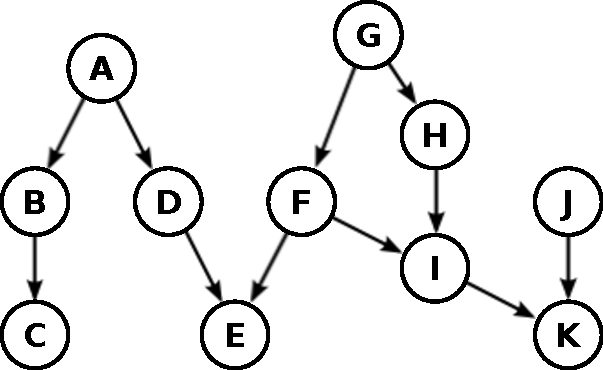
\epsfig{file=figures/Tasks.pdf,width=0.5\textwidth}}
    \caption{A set of tasks (circles) and their dependencies (arrows).
        The arrows indicate the direction of the dependency, i.e.~an
        arrow from task $A$ to task $B$ indicates that task $B$ depends
        on task $A$.
        Tasks $A$, $G$, and $J$ have no unsatisfied dependencies and
        can therefore be executed.
        Once task $G$ has completed, tasks $F$ and $H$ become available,
        and task $E$ only becomes available once both tasks $D$ and $F$
        have completed.}
    \label{fig:Tasks}
\end{figure}

One of the first implementations of a task-based parallel programming
systems is Cilk \cite{ref:Blumofe1995}, an extension to the C
programming language which allows function calls to be ``spawned''
as new tasks.
Dependencies are enforced by the {\tt sync} keyword, which
forces a thread to wait for all the tasks that it spawned
to complete.
Although simple to use, this implicit dependency management
limits the types of DAGs that can be represented, i.e.~for
the example in \fig{Tasks}, using such a spawning model
would create implicit dependencies between the lowest-level
tasks $C$, $E$, and $K$.\footnote{
The main thread spawns tasks $A$, $G$ and $J$, $A$ spawns $B$ and $D$,
$G$ spawns $F$, $H$, and then $I$, $B$ spawns $C$.
The main thread then has to {\tt sync} for $A$, $G$, and $J$,
and thus implicitly all their spawned tasks, before executing
$E$ and $K$.}

In SMP superscalar \cite{ref:Perez2008}, StarPU \cite{ref:Augonnet2011},
QUARK \cite{ref:Yarkhan2011}, and KAAPI \cite{ref:Gautier2007}
the programmer specifies
what shared data each task will access, and how that data will
be accessed, e.g.~read, write, or read-write access.
The dependencies between tasks are then generated
automatically by the runtime system, assuming that the
data must be accessed and updated in the order in which
the tasks are generated.
StarPU also provides an interface for specifying additional
dependencies explicitly.
Intel's Threading Building Blocks (TBB)
\cite{ref:Reinders2010}
provide task-based parallelism using C++ templates.
Dependencies are handled either by explicitly waiting
for spawned tasks, or by explicitly manipulating
task reference counters.

Finally, the very popular OpenMP standard provides some basic support
for spawning tasks, similar to Cilk, as of version 3.0
\cite{ref:OpenMP2008}.
OmpSs \cite{ref:Duran2011} extends this scheme with automatic
dependency generation as in SMP superscalar, of which it
is a direct descendant, along with
the ability to explicitly wait on certain tasks.

In all of these systems, the tasks are only aware of a single
type of relationship between each other, i.e. dependencies, which
specify a strict ordering between two tasks.
In many cases, however, the task ordering need not necessarily
be this strict.
Consider the case of two tasks that update some shared resource
in an order-independent way, e.g. when accumulating a result in
a shared variable, or exclusively writing to an output file.
In order to avoid concurrent access to that resource, it is
imperative that the execution of both tasks do not overlap,
yet the order in which the tasks are executed is irrelevant.
In the following, such a relationship will be referred to
as a ``conflict'' between two tasks.
\fig{TaskConflicts} shows a task graph with conflicting tasks
joined by thick dashed lines.
None of tasks $F$, $H$, and $I$ can be executed concurrently,
i.e. they must be serialized, yet in no particular order.

In dependency-only systems, such conflicts can be modelled
with dependencies, which enforce a pre-determined arbitrary
ordering on conflicting tasks.
This unnecessary restriction on the order
in which tasks can be scheduled can severely limit the
parallelizability of a computation, especially in the presence
of multiple conflicts per task.
Both \citeN{ref:Ltaief2012} and \citeN{ref:Agullo2013} note
this problem in their respective implementations of the Fast Multipole
Method (FMM), in which forces computed in different tasks are
accumulated on a set of particles.

Conflicts can be modeled directly as exclusive locks on a shared resource
which have to be obtained by a task before it can execute.
Thus, in \fig{TaskConflicts}, before executing, task $F$ has
to obtain an exclusive lock on the resource associated with
the conflict between tasks $F$, $H$, and $I$.
While task $F$ is being executed, neither $H$ nor $I$ can 
lock the same resource, and therefore will not execute until
task $F$ is done and the lock has been released.

In order to be of practical use, and to scale well with modern
multi-core shared-memory architectures, any task scheduler
implementing constraints must be:
\begin{itemize}
    \item {\em Correct}: All constraints, i.e.~dependencies and
        conflicts, must be correctly enforced,
    \item {\em Fast}: The overheads associated with task management
        should be as small as possible,
    \item {\em Memory/cache-efficient}: Tasks accessing similar
        sets of data should be preferentially executed on the
        same core to preserve memory/cache locality as far as possible, and
    \item {\em Parallel-efficient}: Tasks should be executed in an order
        that sufficient work is available for all computational
        threads at all times.
\end{itemize}
\noindent This paper presents QuickSched, a framework for task-based
parallel programming with constraints, which aims to achieve
all of these goals.
Section~2 describes the underlying algorithms and data structures,
and Section~3 describes their specific implementation in QuickSched.
Section~4 presents two test-cases:
\begin{enumerate}
    \item The tiled QR
    decomposition described in \cite{ref:Buttari2009} and for
    which the QUARK scheduler was originally developed, and
    \item A task-based Barnes-Hut tree-code to compute the
    gravitational N-body problem similar to the FMM codes
    of \citeN{ref:Ltaief2012} and \citeN{ref:Agullo2013},
\end{enumerate}
These real-world examples show how QuickSched can be used in practice,
and can be used to assess its efficiency.
Section~5 concludes with some general observations and future work
directions.

\begin{figure}
    \centerline{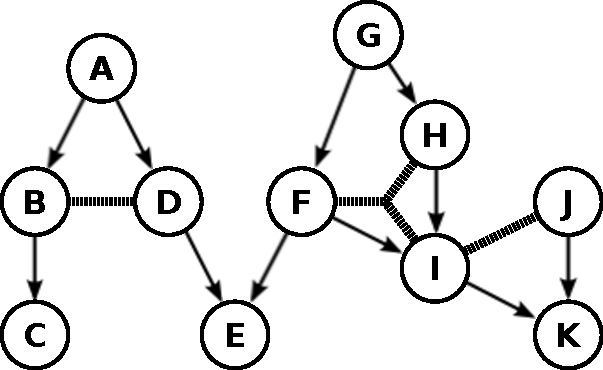
\epsfig{file=figures/TaskConflicts.pdf,width=0.5\textwidth}}
    \caption{Task graph with conflicts (thick dashed lines).
        If two or more tasks are joined by a conflict, they cannot be
        executed concurrently, i.e. tasks $B$ and $D$ cannot be run an
        the same time.
        Tasks belonging to different conflicting sets, e.g. tasks $B$
        and $F$, or tasks $F$ and $J$, however, can be executed
        concurrently.}
    \label{fig:TaskConflicts}
\end{figure}


\section{Data Structures and Algorithms}

The QuickSched task scheduler consist of four main
objects types: {\em task}, {\em resource}, {\em scheduler},
and {\em queue}.

The task and resource objects are used
to model the computation, i.e. the work that is to be done
and the data on which it will be done, respectively.
The scheduler and queue objects manage
how the work is done, i.e. which tasks get scheduled
where and when, respectively.

\begin{figure}
    \centerline{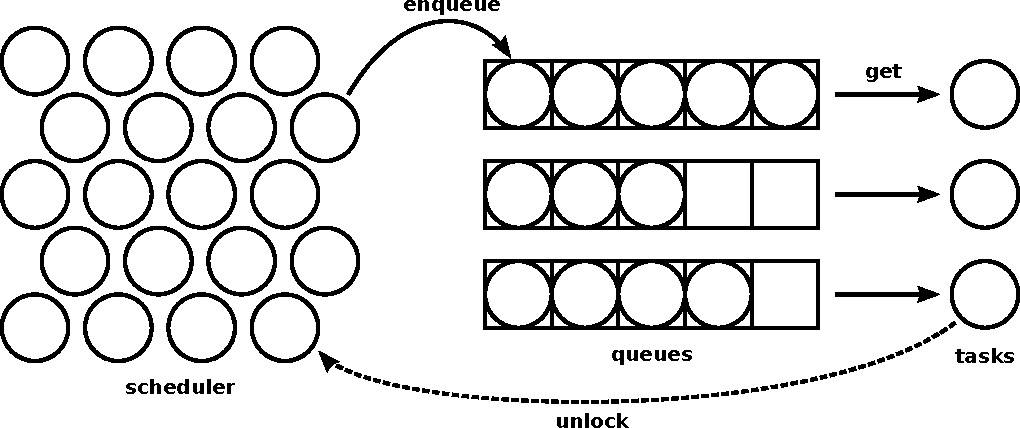
\epsfig{file=figures/QSched.pdf,width=0.7\textwidth}}
    \caption{Schematic of the QuickSched task scheduler.
        The tasks (circles) are stored in the scheduler (left).
        Once a task's dependencies have been resolved, the task
        is moved to one of the task queues.
        Tasks that are not involved in any active conflicts
        are then taken from the queues by the different
        computational threads and executed.
        After execution, their dependent tasks are unlocked
        in the scheduler (dashed arrow).}
    \label{fig:QSched}
\end{figure}

The division of labor regarding {\em correctness}
between the scheduler and
the queue objects is illustrated in \fig{QSched}.
The scheduler holds the tasks and is in charge
of managing {\em dependencies}.
Once a task has no unresolved dependencies, it is passed
on to a queue object.
The queue object, on the other hand, is in charge
of managing {\em conflicts}.
Computational threads can query a queue and will
receive only tasks for which all conflicts have been
resolved, i.e. for which all necessary resources could be 
exclusively locked.

There is also a division of responsibilities regarding
{\em efficiency} between the scheduler and the queue
objects.
The tasks in each queue are grouped according to the resources
they use, i.e. all the tasks in the same queue use a
similar set of resources.
The underlying assumption is that each computational
thread will preferentially access the same queue for tasks.
If the tasks in the queue share the same set of resources,
in increases the probability of said resources already
being present in the thread's cache, thus increasing
{\em memory efficiency}.
The scheduler is in charge of selecting the most appropriate
queue for each task, based on information stored in each task
on which resources are used.
Given a set of tasks with similar resources for which all
dependencies are resolved, the queue then decides which
tasks to prioritize.
This decision is made based on the length of the critical
path of the dependencies of each task.

The following subsections describe these four object types
in detail, as well as their operations.


\subsection{Tasks}
\label{sec:tasks}

A task consists of the following data structure, in C-like pseudo-code:

\begin{center}\begin{minipage}{0.9\textwidth}
    \begin{lstlisting}
struct task {
  int type, wait;
  void *data;
  struct task **unlocks;
  struct resource **locks, **uses;
  int size_data, nr_unlocks, nr_locks, nr_uses;
  int cost, weight;
  };
    \end{lstlisting}
\end{minipage}\end{center}
\noindent where the {\tt data}, {\tt unlocks}, {\tt locks},
and {\tt uses} arrays are pointers to the contents of other
arrays, i.e.~they are not allocated individually.

What the task does is determined by the {\tt type}
field, e.g.~which can be mapped to any particular function,
and the {\tt data} pointer which points to an array of
{\tt size\_data} bytes containing data specific to the task,
e.g.~the parameters for a specific function call.
Both fields are application-specific and therefore not
important for the scheduler itself.

The {\tt unlocks} field points to the first element of
an array of {\tt nr\_unlocks} pointers to other tasks.
These pointers represent the dependencies in reverse:
if task $B$ depends on task $A$, then task $A$ {\em unlocks}
task $B$.
The unlocks therefore follow the direction of the arrows
in \figs{Tasks}{TaskConflicts}.
Conversely, {\tt wait} is the number of unresolved dependencies
associated with this task, i.e.~the number of unexecuted tasks
that unlock this task.
Given an array of {\tt N} tasks, the wait-counters can
be set as follows:
\begin{center}\begin{minipage}{0.9\textwidth}
    \begin{lstlisting}
int j, k;
for ( k = 0 ; k < N ; k++ )
  tasks[k].wait = 0;
for ( k = 0 ; k < N ; k++ )
  for ( j = 0 ; j < tasks[k].nr_unlocks ; j++ )
    tasks[k].unlocks[j]->wait += 1;
    \end{lstlisting}
\end{minipage}\end{center}

The {\tt locks} field of each task points to the first element of
an array of {\tt nr\_locks} pointers to {\em resources}
for which exclusive locks must be obtained for the task
to execute.
Each locked resource represents a task conflict.
Similarly, {\tt uses} points to the first element of
an array of {\tt nr\_uses} pointers to resources which
will be used, but need not be locked.

Finally, {\tt cost} and {\tt weight} are measures
for the relative computational cost of this task, and the
relative cost of the critical path following the
dependencies of this task, respectively.
The task weights can be computed by first sorting
the tasks topologically according to their dependencies, i.e.
as per \citeN{ref:Kahn1962}:
\begin{center}\begin{minipage}{0.9\textwidth}
    \begin{lstlisting}
int top[N], j, k, sorted = 0, maxweight;
set the task waits as described above.
for ( k = 0 ; k < N ; k++ )
  if ( tasks[k].wait == 0 )
    top[ sorted++ ] = k;
for ( k = 0 ; k < sorted ; k++ )
  for ( j = 0 ; j < tasks[ top[k] ].nr_unlocks ; j++ )
    if ( ( tasks[ top[k] ].unlock[j]->wait -= 1 ) == 0 )
      top[ sorted++ ] = k;
if ( k < N )
  error( "Circular dependencies detected." );
    \end{lstlisting}
\end{minipage}\end{center}
\noindent where the array {\tt top} contains the task indices
in topological order. 
The test in line~10 is a convenient check if the tasks and their
dependencies actually do form an acyclic graph.
The weights themselves are then computed as follows
\begin{center}\begin{minipage}{0.9\textwidth}
    \begin{lstlisting}
for ( k = N-1 ; k >= 0 ; k-- ) {
  for ( w = 0 , j = 0 ; j < tasks[ top[k] ].nr_unlocks ; j++ ) {
    tasks[ top[k] ].unlock[j]->wait += 1;
    w = max( tasks[ top[k] ].unlock[j]->weight , w );
    }
  tasks[ top[k] ].weight = tasks[ top[k] ].cost + w;
  }
    \end{lstlisting}
\end{minipage}\end{center}
\noindent where the tasks are traversed in reverse
topological order, computing the recursive weight as the sum of the
task cost and the maximum weight of the tasks it unlocks (line~6),
and recomputing the task waits at the same time (line~3).


\subsection{Resources}

Resources consist of the following data structure:
\begin{center}\begin{minipage}{0.9\textwidth}
    \begin{lstlisting}
struct resource {
  struct resource *parent;
  volatile int lock, hold;
  int owner;
  };
    \end{lstlisting}
\end{minipage}\end{center}

The {\tt parent} field, which points to another resource, is
used to create hierarchical resources, i.e.~resources
that are themselves subsets of larger resources.
This can be useful, e.g.~in the context of particle simulations
described in the next section, where particles are sorted
into hierarchical cells which are used at different levels.
The {\tt owner} field is the ID of the queue to which this
resource has been preferentially assigned.

The {\tt lock} field is either {\tt 0} or {\tt 1} and indicates
whether this resource is currently in use, i.e.~{\em locked}.
To avoid race conditions, this value should only be tested
and set using atomic instructions.
The {\tt hold} field is a counter indicating how many
sub-resources of the current resource are locked.
If a resource's hold counter is not zero, then it is
{\em held} and cannot be locked.
Likewise, if a resource is locked, it cannot be held
(see \fig{Resources}).

\begin{figure}
    \centerline{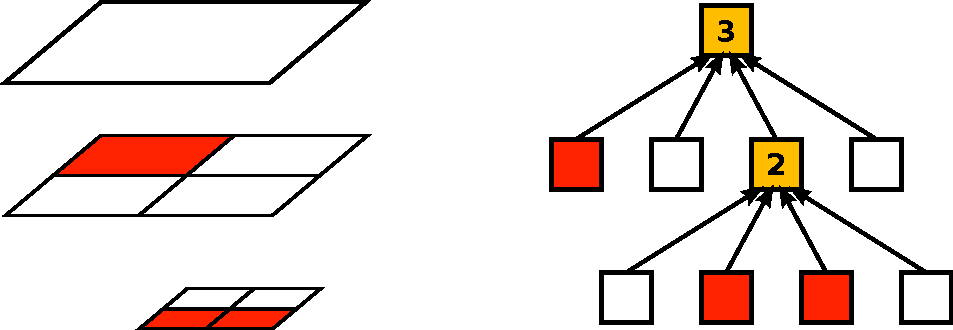
\epsfig{file=figures/Resources.pdf,width=0.6\textwidth}}
    \caption{A hierarchy of cells (left) and the hierarchy of
        corresponding hierarchical resources at each level.
        Each square on the right represents a single resource, and
        arrows indicate the resource's parent.
        Resources colored red are locked, resources colored orange
        are held, where the number in the square indicates the
        value of the hold counter.}
    \label{fig:Resources}
\end{figure}

Incrementing the hold counter of the resource can be implemented
as follows:
\begin{center}\begin{minipage}{0.9\textwidth}
    \begin{lstlisting}
void resource_hold ( struct resource *r ) {
  if ( atomic_cas( &r->lock , 0 , 1 ) != 0 )
    return 0;
  atomic_inc( &r->hold );
  r->lock = 0;
  return 1;
  }
    \end{lstlisting}
\end{minipage}\end{center}
\noindent where {\tt atomic\_cas(val,old,new)} is an atomic
compare-and-swap operation that sets {\tt val} to {\tt new}
if it is currently equal to {\tt old}.
Similarly, {\tt atomic\_inc(val)} increments {\tt val} by one
atomically.
The resource's {\tt lock} is used to check if the resource
is already locked (line 2), and it is held while {\tt hold}
is incremented, to avoid overlapping hold/lock operations.
If the resource can be locked, the hold counter is incremented
atomically (line~4), and the lock is released (line~5),
returning {\tt 1} or {\tt 0} if the resource could be held
or not, respectively.

The locking procedure itself is implemented as follows:
\begin{center}\begin{minipage}{0.9\textwidth}
    \begin{lstlisting}
void resource_lock ( struct resource *r ) {
  struct resource *up, *top;
  if ( r->hold && atomic_cas( &r->lock , 0 , 1 ) != 0 )
    return 0;
  if ( r->hold ) {
    r->lock = 0;
    return 0;
    }
  for ( up = r->parent ; up != NULL ; up = up->parent ) {
    if ( !resource_hold( up ) )
      break;
  if ( ( top = up ) != NULL ) {
    for ( up = r->parent ; up != top , up = up->parent )
      atomic_dec( &up->hold );
    r->lock = 0;
    return 0;
    }
  else
    return 1;
  }
    \end{lstlisting}
\end{minipage}\end{center}
\noindent where in line~3 the resource is first locked if it
is not held.
Due to a possible race condition when holding the resource,
the {\tt hold} counter must checked again once the resource
has been locked (line~5).
In lines~9--11 the hold counters of the hierarchical parents
are incremented using the procedure described earlier.
If this process fails at any point (line~12), the
previously set hold counters are decremented (lines~13--14)
and the lock is released (line~15).
The procedure then returns {\tt 1} or {\tt 0} if the resource
could be locked or not, respectively.

Finally, unlocking a resource is relatively straight-forward:
\begin{center}\begin{minipage}{0.9\textwidth}
    \begin{lstlisting}
void resource_unlock ( struct resource *r ) {
  struct resource *up;
  r->lock = 0;
  for ( up = r->parent ; up != NULL ; up = up->parent ) {
    atomic_dec( &up->hold );
  }
    \end{lstlisting}
\end{minipage}\end{center}
\noindent where the resource itself is unlocked (line~3)
and the hold counters of all of its hierarchical parents
are decremented (lines~4--5).


\subsection{Queues}

The main job of the task queues is, given a set of ready tasks,
to find the task with maximum weight whose resources can all
be locked, and to do so as efficiently as possible.

One possible strategy would be to maintain an array of tasks
sorted by their weights, and to traverse that list in descending
order, trying to lock the resources of each task, until
a lockable task is found, or returning a failure otherwise.
Although this would return the best possible task, it
requires maintaining a sorted list in which inserting
or removing an entry is in \oh{n} for $n$ elements.
Using an unsorted array would require only \oh{1} operations for
insertion and deletion, but is undesirable as it completely
ignores the task weights.

As a compromise, the queue stores the tasks in an array
organized as a max-heap, i.e.~where the $k$th entry is ``larger''
than both the $2k+1$st and the $2k+2$nd entry,
with the task with maximum weight
in the first position.
Maintaining this heap structure thus requires \oh{\log n}
operations for both insertion and deletion, i.e. for the
bubble-up and trickle-down operations respectively.

The array of tasks is then traversed as if it were sorted,
returning the first task that can be locked.
Although the first task in the array will be the task with
maximum weight, the following tasks are only loosely ordered,
where the $k$th of $n$ tasks has a larger weight than at least
$\lfloor n/k\rfloor -1$ other tasks.

The data structure for the queue is thus defined as follows:
\begin{center}\begin{minipage}{0.9\textwidth}
    \begin{lstlisting}
struct queue {
  struct task **tasks;
  int count, lock;
  };
    \end{lstlisting}
\end{minipage}\end{center}
\noindent where {\tt tasks} is an array of {\tt count} pointers
to the tasks in max-heap order, and {\tt lock} is used to
guarantee exclusive access to the queue.

Inserting a task in the queue is relatively straight-forward:
\begin{center}\begin{minipage}{0.9\textwidth}
    \begin{lstlisting}
void queue_put ( struct queue *q , struct task *t ) {
  while ( atomic_cas( q->lock , 0 , 1 ) != 0 );
  q->tasks[ q->count++ ] = t;
  bubble-up the q->count-1st entry of q->tasks.
  q->lock = 0;
  }
    \end{lstlisting}
\end{minipage}\end{center}
\noindent where the loop in line~2 spins until an exclusive
lock on the queue can be obtained.
The task is added to the end of the heap array (line~3)
and the heap order is fixed (line~4).
Before returning, the lock on the queue is released (line~5).

Obtaining a task from the queue can be implemented as follows:
\begin{center}\begin{minipage}{0.9\textwidth}
    \begin{lstlisting}
struct task *queue_get ( struct queue *q ) {
  struct task *res = NULL;
  int j, k;
  while ( atomic_cas( q->lock , 0 , 1 ) != 0 );
  for ( k = 0 ; k < q->count ; k++ ) {
    for ( j = 0 ; j < q->tasks[k]->nr_locks ; j++ )
      if ( !resource_lock( q->tasks[k]->lock[j] ) )
        break;
    if ( j < q->tasks[k]->nr_locks )
      for ( j = j-1 ; j >= 0 ; j-- )
        resource_unlock( q->tasks[k]->lock[j] );
    else
      break;
    }
  if ( k < q->count ) {
    res = q->tasks[k];
    q->tasks[k] = q->tasks[ --q->count ];
    trickle-down the kth entry of q->tasks.
    }
  q->lock = 0;
  return res;
  }
    \end{lstlisting}
\end{minipage}\end{center}
\noindent where as with the queue insertion, the queue is first
locked for exclusive access (line~4).
The array of task pointers is then traversed in heap order (line~5),
locking the resources of each task (lines~6--8).
If any of these locks fail (line~9), the locks that were obtained
are released (lines~10--11), otherwise, the traversal is aborted
(line~13).
If all the locks on a task could be obtained (line~15), the
task pointer is replaced by the last pointer in the heap (line~17)
and the heap order is restored (line~18).
Finally, the queue lock is released (line~19) and the locked task
or, if no lockable task could be found, {\tt NULL} is returned.


\subsection{Scheduler}

The scheduler object is used as the main interface to the
QuickSched task scheduler, and as such contains the instances
of the other three object types:
\begin{center}\begin{minipage}{0.9\textwidth}
    \begin{lstlisting}
struct qsched {
  struct task *tasks;
  struct queue *queues;
  struct resource *res;
  int nr_tasks, nr_queues, nr_resources;
  volatile int waiting;
  };
    \end{lstlisting}
\end{minipage}\end{center}
\noindent where the only additional field {\tt waiting} is
used to keep track of the number of tasks that have not been
executed.
Note that for brevity, and to avoid conflicts with the naming
schemes of other standard libraries, the type name {\tt qsched}
is used for the scheduler data type.

The tasks are executed as follows:
\begin{center}\begin{minipage}{0.9\textwidth}
    \begin{lstlisting}
void qsched_run ( qsched *s , void (*fun)( int , void * ) ) {
  qsched_start( s );
  #pragma omp parallel
  {
    int qid = omp_get_thread_num() % s->nr_queues;
    struct task *t;
    while ( ( t = qsched_gettask( s , qid ) ) != NULL ) {
      fun( t->type , t->data );
      qsched_done( s , t );
      }
    }
  }
    \end{lstlisting}
\end{minipage}\end{center}
\noindent where {\tt qsched\_start} initializes the tasks and
fills the queues (line~1).
For simplicity, OpenMP \cite{ref:Dagum1998}, which is available
for most compilers, is used to create a parallel section
in which the code between lines~4 and~11 is executed
concurrently.
The parallel section consists of a loop (lines~7--10) in
which a task is acquired via {\tt qsched\_gettask}
and its type and data are passed to a user-supplied
{\em execution function} {\tt fun}.
Once the task has been executed, it is returned to the
scheduler via the function {\tt qsched\_done}, i.e.~to
unlock its resources and unlock dependent tasks.
The loop terminates when the scheduler runs out of tasks,
i.e.~when {\tt qsched\_gettask} returns {\tt NULL}, and
the function exits once all the threads have exited their
loops.

At the start of a parallel computation, {\tt qsched\_start}
identifies the tasks that have no dependencies and sends them
to queues:
\begin{center}\begin{minipage}{0.9\textwidth}
    \begin{lstlisting}
void qsched_start ( qsched *s ) {
  sort out pointers in tasks.
  set the task waits and weights.
  s->waiting = s->nr_tasks;
  for ( k = 0 ; k < s->nr_tasks && s->tasks[tid[k]].wait == 0 ; k++ )
    qsched_enqueue( s , &s->tasks[tid[k]] );
  }
    \end{lstlisting}
\end{minipage}\end{center}
\noindent where line~2 sets the {\tt unlocks}, {\tt locks},
and {\tt uses} pointers in the tasks.
The operations in line~3 are described in \sect{tasks}.
The function {\tt qsched\_enqueue} tries to identify the best
queue for a given task by looking at which queues last used
the resources used and locked by the task, e.g.:
\begin{center}\begin{minipage}{0.9\textwidth}
    \begin{lstlisting}
void qsched_enqueue ( qsched *s , struct task *t ) {
  int k, qid, score[ s->nr_queues ];
  for ( k = 0 ; k < s->nr_queues ; k++ )
    score[k] = 0;
  for ( j = 0 ; j < t->nr_locks ; j++ )
    score[ t->locks[j]->owner ] += 1;
  for ( j = 0 ; j < t->nr_uses ; j++ )
    score[ t->uses[j]->owner ] += 1;
  for ( qid = 0 , k = 1 ; k < s->nr_queues ; k++ )
    if ( score[k] > score[qid] )
      qid = k;
  queue_put( &s->queues[qid] , t );
  }
    \end{lstlisting}
\end{minipage}\end{center}
\noindent where the array {\tt score} keeps a count of the
task resources ``owned'', or last used, by each queue.
In lines~9--11 the queue with the highest such score is 
chosen on which the task is then put (line~12).

The function {\tt qsched\_gettask} fetches a task from
one of the queues:
\begin{center}\begin{minipage}{0.9\textwidth}
    \begin{lstlisting}
struct task *qsched_gettask ( qsched *s , int qid ) {
  struct task *res = NULL;
  int k;
  while ( s->waiting ) {
    if ( ( res = queue_get( s->queues[qid] ) ) == NULL ) {
      loop over all other queues in random order with index k
        if ( ( res = queue_get( s->queues[k] ) ) != NULL )
          break;
      }
    else
      break;
    }
  if ( res != NULL && s->reown ) {
    for ( k = 0 ; k < res->nr_locks ; k++ )
      res->locks[k]->owner = qid;
    for ( k = 0 ; k < res->nr_uses ; k++ )
      res->uses[k]->owner = qid;
    }
  return res;
  }
    \end{lstlisting}
\end{minipage}\end{center}
\noindent where the parameter {\tt qid} is the index of the
preferred queue.
If the queue is empty, or all of the tasks in that queue had
unresolved conflicts, the scheduler uses {\em work stealing}
\cite{ref:Blumofe1999}, i.e.~it loops over all other queues
in a random order (line~6) and tries to get a task from them
(line~7).
If a task could be obtained from any queue and task re-owning
is switched on (line~13),
the resources it locks and uses are marked as now being owned
by the preferred queue (lines~14--17).
Finally, the task, or {\tt NULL} if no task could be obtained,
is returned.

The final step in a task's life cycle is, on completion,
to unlock the resources and tasks which depend on it.
This is handled by the function {\tt qsched\_done}:
\begin{center}\begin{minipage}{0.9\textwidth}
    \begin{lstlisting}
void qsched_done ( qsched *s , struct task *t ) {
  int k;
  for ( k = 0 ; k < t->nr_locks ; k++ )
    resource_unlock( t->locks[k] );
  for ( k = 0 ; k < t->nr_unlocks ; k++ )
    if ( atomic_dec( &t->unlocks[k]->wait ) == 1 )
      qsched_enqueue( s , t->unlocks[k] );
  atomic_dec( &s->waiting );
  }
    \end{lstlisting}
\end{minipage}\end{center}
\noindent If any of the unlocked tasks' wait counters
goes to zero (line~6), then the unlocked task is ready to
run and is immediately dispatched via {\tt qsched\_enqueue},
as described earlier.
Once all the dependent tasks have been unlocked, the
{\tt waiting} counter is decremented (line~8).


\section{User Interface}

The algorithms, as described in the previous section, have
all been implemented as part of the Open-Source C-language
QuickSched library.\footnote{\url{http://sourceforge.net/projects/quicksched/}}
This section describes the interface functions and how they
are called, and the following section contains
examples of how QuickSched can be used.

As mentioned previously, the {\tt qsched} object is the main
interface to the task scheduler.
As such, it provides functionality for task and resource
creation, for assigning resources to tasks, either as locks
or uses, and for assigning dependencies between tasks.
The tasks and resources themselves are opaque to the
user, and handles of the types {\tt qsched\_task\_t}
and {\tt qsched\_res\_t} are used instead.

The main functions for setting up the scheduler are:
\begin{itemize}
    \item {\tt void qsched\_init( struct qsched *s , int nr\_queues , int flags )} \\
        Initializes a {\tt qsched} object with the given number of queues.
        The {\tt flags} parameter can be set to any bitwise or combination
        of {\tt qsched\_flag\_none},
        {\tt qsched\_flag\_yield}, and {\tt qsched\_flag\_pthread},
        which are described further below.
        This function must be called before any of the other
        functions are used.
        \vspace{1mm}
    \item {\tt void qsched\_free( struct qsched *s )} \\
        Releases all the memory and other resources allocated by the
        given {\tt qsched} object.
        After this function has been called, the {\tt qsched} will
        need to be re-initialized for reuse.
        \vspace{1mm}
    \item {\tt void qsched\_reset( struct qsched *s )} \\
        Clears the tasks and resources in the given {\tt qsched},
        but does not release the allocated memory or change
        the number of queues.
        \vspace{1mm}
    \item {\tt qsched\_task\_t qsched\_addtask( struct qsched *s , int type , unsigned int flags , void *data , int data\_size , int cost )} \\
        Creates a new task within the given {\tt qsched} and returns
        its handle.
        The {\tt type} and {\tt data} field are copied into the {\tt qsched}
        and passed to the execution function when the {\tt qsched} is run.
        The parameter flags is either {\tt task\_flag\_none} or
        {\tt task\_flag\_virtual}.
        Tasks marked as virtual do not have any action associated with them,
        e.g. they are used only to group or otherwise dependencies, and
        are not passed to the execution function in {\tt qsched\_run}.
        \vspace{1mm}
    \item {\tt qsched\_res\_t qsched\_addres( struct qsched *s , int owner , qsched\_res\_t parent )} \\
        Creates a new resource within the given {\tt qsched} and returns
        its handle.
        The owner field is the initial queue ID to which this resource
        should be assigned, or {\tt qsched\_owner\_none}.
        The {\tt parent} field is the handle of the hierarchical parent of
        the new resource or {\tt qsched\_res\_none} if the resource
        has no hierarchical parent.
        \vspace{1mm}
    \item {\tt void qsched\_addlock( struct qsched *s , qsched\_task\_t t , qsched\_res\_t res )} \\
        Append the resource {\tt res} to the task {\tt t}'s list of
        locks.
        The task {\tt t} will then conflict with any other task that
        also locks the resource {\tt res}, its hierarchical parents, or
        any resource hierarchically below it.
        \vspace{1mm}
    \item {\tt void qsched\_adduse( struct qsched *s , qsched\_task\_t t , qsched\_res\_t res )} \\
        Similar to {\tt qsched\_addlock}, yet the resource is only used and
        is not part of a conflict.
        This information is used when assigning tasks to specific queues.
        \vspace{1mm}
    \item {\tt void qsched\_addunlock( struct qsched *s , qsched\_task\_t ta , qsched\_task\_t tb )} \\
        Appends the task {\tt tb} to the list of tasks that the task {\tt ta}
        unlocks.
        The task {\tt tb} then depends on the task {\tt ta}.
        \vspace{1mm}
    \item {\tt void qsched\_run( struct qsched *s , int nr\_threads , qsched\_funtype fun )} \\
        Executes the tasks in the given {\tt qsched} using {\tt nr\_threads}
        threads via the execution function {\tt fun}, as described in the
        previous section.
        Once a {\tt qsched} has been initialized and filled with
        tasks and resources, it can be run more than once.
        \vspace{1mm}
\end{itemize}

The library can be compiled to use OpenMP and/or the
{\tt pthreads} library \cite{ref:Pthreads1995}.
OpenMP is the default, but calling {\tt qsched\_init} with
either the {\tt qsched\_flag\_yield}
or the {\tt qsched\_flag\_pthread} switches to using {\tt pthreads},
if available, for the parallel loop.

OpenMP has the advantage of being available for most compilers
and also potentially providing some extra platform-specific
scheduling features, e.g.~optimal thread location and/or affinity,
and of integrating seamlessly with other parallel parts of the
user application.
The disadvantage of using OpenMP is that it does not provide
any mechanism for yielding a thread if no tasks are available,
i.e. the main loop in {\tt qsched\_gettask}, described in the
previous section, will spin until a task becomes available.
This may be a problem if other parts of the user application
are running concurrently in the background.
Calling {\tt qsched\_init} with the {\tt qsched\_flag\_yield}
forces the use of {\tt pthreads} and uses conditional variables
to wait for a new task to be enqueued if obtaining a task
from any of the queues fails.
This relinquishes the waiting computational thread for other
processes.


\section{Validation}

This section presents two test cases showing
how QuickSched can be used in real-world applications, and
providing benchmarks to assess its efficiency and scalability.

The first test is the tiled QR decomposition originally
described in \citeN{ref:Buttari2009}, which has been used as a benchmark
by other authors \cite{ref:Agullo2009b,ref:Badia2009,ref:Bosilca2012}.
This example only requires dependencies and is presented 
as a point of comparison to existing task-based parallel
programming infrastructures.

The second example is a Barnes-Hut tree-code, a problem
similar to the Fast Multipole Method described in both
\citeN{ref:Ltaief2012} and \citeN{ref:Agullo2013}.
This example shows how conflicts, modeled
via hierarchical resources, can be useful.

The source code of both examples is distributed with the
QuickSched library, along with scripts to run the benchmarks
and generate the plots used in the following.
All examples were compiled with gcc v.\,4.8.1 using the
{\tt -O2 -march=native} flags and run on a 
tests were run on a 64-core AMD Opteron 6376 machine running
at 2.6\,GHz.


\subsection{Task-Based QR Decomposition}

\citeN{ref:Buttari2009} introduced the concept of using task-based
parallelism for tile-based algorithms in numerical linear algebra,
presenting parallel codes for the Cholesky, LU, and QR
decompositions.
These algorithms are now part of the PLASMA and MAGMA
libraries for parallel linear algebra \cite{ref:Agullo2009}.
The former uses the QUARK task scheduler, which was originally
designed for it, while the latter currently uses the StarPU
task scheduler.

\begin{figure}
    \centerline{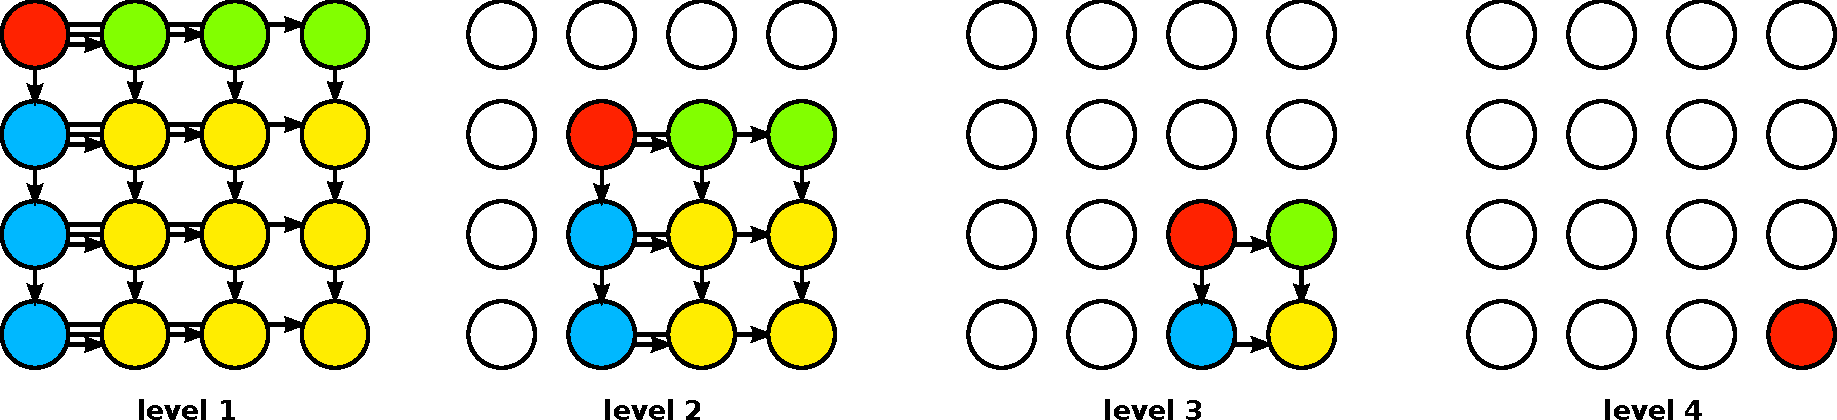
\epsfig{file=figures/QR.pdf,width=0.8\textwidth}}
    \caption{Task-based QR decomposition of a matrix consisting
        of $4\times 4$ tiles.
        Each circle represents a tile, and its color represents
        the type of task on that tile at that level.
        Empty circles have no task associated with them.
        The arrows represent dependencies at each level, and
        tasks at each level also implicitly depend on the
        task at the same location in the previous level.}
    \label{fig:QR}
\end{figure}

The tiled QR factorization is based on four basic tasks,
or kernels, as shown in \fig{QR}.
For a matrix consisting of $N\times N$ tiles, $N$ passes,
or levels, are computed, each computing a column and row of the QR
decomposition.
The tasks can be defined in terms of the tuples $(i,j,k)$,
where $i$ and $j$ are the row and column of the tile, respectively,
and $k$ is its level:

\begin{center}
    \begin{tabular}{llll}
        Task & where & depends on task(s) & locks tile(s) \\
        \hline
        
\epsfig{file=figures/TaskRed.pdf,height=9pt} DGEQRF & $i=j=k$ & $(i,j,k-1)$ & $(i,j)$ \\
        
\epsfig{file=figures/TaskGreen.pdf,height=9pt} DLARFT & $i=k$, $j>k$ & $(i,j,k-1)$, $(k,k,k)$ & $(i,j)$ \\
        
\epsfig{file=figures/TaskBlue.pdf,height=9pt} DTSQRF & $i>k$, $j=k$ & $(i,j,k-1)$, $(i-1,j,k)$ & $(i,j)$, $(j,j)$ \\
        
\epsfig{file=figures/TaskYellow.pdf,height=9pt} DSSRFT & $i>k$, $j>k$ & $(i,j,k-1)$, $(k,j,k)$, $(i,k,k)$ & $(i,j)$ \\
        \hline
    \end{tabular}
\end{center}

\noindent where the task names are the BLAS-like operation
performed on the given tiles.
Every task depends on the task at the same position and the
previous level, i.e.~the task $(i,j,k)$ always depends on
$(i,j,k-1)$ for $k>1$.
Each task also modifies its own tile $(i,j)$, and the DTSQRF
task additionally modifies the lower triangular part of the $(j,j)$th tile.

\begin{figure}
\begin{center}\begin{minipage}{0.9\textwidth}
    \begin{lstlisting}
enum { tDGEQRF , tDLARFT , tDTSQRF , tDSSRFT };
void make_tasks ( struct qsched *s , int m , int n ) {
  int i, j, k, data[3];
  qsched_task_t tid[ m*n ], tid_new;
  qsched_res_t rid[ m*n ];
  for ( k = 0 ; k < m*n ; k++ ) {
    tid[k] = qsched_task_none;
    rid[k] = qsched_addres( s , qsched_res_none );
    }
  for ( k = 0 ; k < m && k < n ; k++ ) {
    /* DGEQRF task at (k,k). */
    data[0] = k; data[1] = k; data[2] = k;
    tid_new = qsched_addtask( s , tDGEQRF , qsched_flags_none ,
      data , sizeof(int)*3 , 2 );
    qsched_addlock( s , tid_new , rid[ k*m + k ] )
    if ( tid[ k*m + k ] != qsched_task_none )
      qsched_addunlock( s , tid[ k*m + k ] , tid_new );
    tid[ k*m + k ] = tid_new;
    for ( j = k+1 ; j < n ; j++ ) {
      /* DLARFT task at (k,j). */
      data[0] = k; data[1] = j; data[2] = k;
      tid_new = qsched_addtask( s , tDLARFT , qsched_flags_none ,
        data , sizeof(int)*3 , 3 );
      qsched_addlock( s , tid_new , rid[ j*m + k ] )
      qsched_addunlock( s , tid[ k*m + k ] , tid_new );
      if ( tid[ j*m + k ] != qsched_task_none )
        qsched_addunlock( s , tid[ j*m + k ] , tid_new );
      tid[ j*m + k ] = tid_new;
      }
    for ( i = k+1 ; i < m ; i++ ) {
      /* DTSQRF task at (i,k). */
      data[0] = i; data[1] = k; data[2] = k;
      tid_new = qsched_addtask( s , tDTSQRF , qsched_flags_none ,
        data , sizeof(int)*3 , 3 );
      qsched_addlock( s , tid_new , rid[ k*m + i ] )
      qsched_addlock( s , tid_new , rid[ k*m + k ] )
      qsched_addunlock( s , tid[ k*m + k ] , tid_new );
      if ( tid[ k*m + i ] != qsched_task_none )
        qsched_addunlock( s , tid[ k*m + i ] , tid_new );
      tid[ k*m + i ] = tid_new;
      for ( j = k+1 ; j < n ; j++ ) {
        /* DSSRFT task at (i,j). */
        data[0] = i; data[1] = j; data[2] = k;
        tid_new = qsched_addtask( s , tDSSRFT , qsched_flags_none ,
          data , sizeof(int)*3 , 5 );
        qsched_addlock( s , tid_new , rid[ j*m + i ] )
        qsched_addunlock( s , tid[ j*m + k ] , tid_new );
        qsched_addunlock( s , tid[ k*m + i ] , tid_new );
        if ( tid[ j*m + i ] != qsched_task_none )
          qsched_addunlock( s , tid[ j*m + i ] , tid_new );
        tid[ j*m + i ] = tid_new;
        }
      }
    }
  }
    \end{lstlisting}
\end{minipage}\end{center}
\caption{Example code to generate the tasks for the tiled
    QR decomposition.}
\label{fig:CodeQR}
\end{figure}

Setting up the dependencies and locks for a matrix of
$m\times n$ tiles is implemented as shown in \fig{CodeQR},
where the $m\times n$ matrix {\tt tid} stores the handles
of the last task at position $(i,j)$ and is initialized with
empty tasks (line~7).
Similarly, {\tt rid} stores the handles of the resources for each
tile of the matrix, which are allocated in line~8.

The following loops mirror the task generation described in
Algorithm~2 of \citeN{ref:Buttari2009}.
For each level {\tt k} (line~10), a DGEQRF task is created
for tile $(k,k)$ (lines~13--14).
A lock is added for the newly created task on the
resource associated with the $(k,k)$th tile (line~15).
If a task exists at that position at the previous level
(line~16), a dependency is added between the old task and
the new (line~17), and the new task is stored in {\tt tid}
(line~18).
The remaining tasks are generated in the same way, with
their respective locks and dependencies.

The execution function for these tasks simply calls the appropriate
kernels on the matrix tiles given by the task data:
\begin{center}\begin{minipage}{0.9\textwidth}
    \begin{lstlisting}
void exec_fun ( int type , void *data ) {
  int *idata = (int *)data;
  int i = idata[0], j = idata[1], k = idata[2];
  switch ( type ) {
    case tDGEQRF:
      DGEQRF( A[i,j] , ... );
      break;
    case tDLARFT:
      DLARFT( A[i,j] , A[i,i] , ... );
      break;
    case tDTSQRF:
      DTSQRF( A[i,j] , A[j,j]... );
      break;
    case tDSSRFT:
      DSSRFT( A[i,j] , A[i,k] , A[k,j] , ... );
      break;
    default:
      error( "Unknown task type." );
    }
  }
    \end{lstlisting}
\end{minipage}\end{center}
\noindent where {\tt A} is the matrix over which the QR
decomposition is executed.

The QR decomposition was computed for a $2048\times 2048$
random matrix using tiles of size $64\times 64$ using QuickSched
as described above.
For the DGEQRF and DLARFT kernels, the respective routines
from the LAPACKE\footnote{\url{http://www.netlib.org/lapack/lapacke.html}}
library were used.
The DTSQRF and DSSRFT kernels were implemented by Sam Townsend
as part of his MSc thesis in Computer Science at Durham University.
For this matrix, a total of 11440 tasks with 32240 dependencies
were generated.

For these tests, OpenMP parallelism and resource re-owning
were used with one queue per core.
The QR decomposition was computed 10 times for each number of
cores, and the average thereof taken for the scaling and
efficiency results in \fig{QRResults}.
The timings are for {\tt qsched\_run}, including the cost of
{\tt qsched\_start}, which does not run in parallel.
Setting up the scheduler, tasks, and resources took, in all
cases, an average of 7.2\,ms.

The same decomposition was implemented using OmpSs v.\,1.99.0,
calling the kernels directly using {\tt \#pragma omp task}
annotations with the respective dependencies, and
the runtime parameters
\begin{quote}
    \tt --disable-yield --schedule=socket --cores-per-socket=16 --num-sockets=4
\end{quote}
\noindent The scaling and efficiency relative to QuickSched are 
shown in \fig{QRResults} as well.
The difference in timings is the result of the different
task scheduling policies, as well as a smaller lag between the
individual tasks, as shown in \fig{QRTasks},
which shows the assignment of the different tasks to cores for the
64 core run.
The most visible difference between both schedulers is that
the DGEQRF tasks (in red) are scheduled as soon as they
become available in QuickSched, thus preventing bottlenecks
near the end of the computation.

\begin{figure}
    \centerline{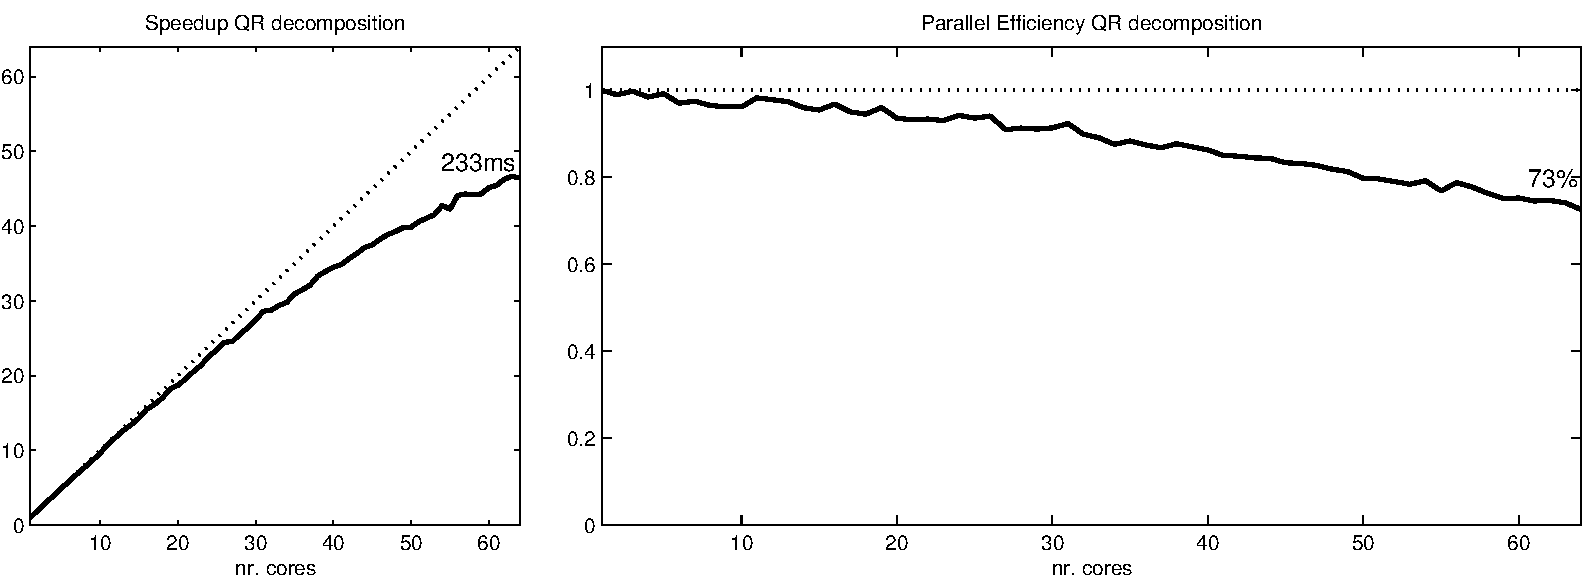
\epsfig{file=figures/QR_scaling.pdf,width=0.9\textwidth}}
    \caption{Strong scaling and parallel efficiency of the tiled QR decomposition
        computed over a $2048\times 2048$ matrix with tiles of size
        $64\times 64$.
        The QR decomposition with QuickSched takes 233\,ms,
        achieving 73\% parallel efficiency, over all 64 cores.
        The scaling and efficiency for OmpSs are computed relative to QuickSched.
        }
    \label{fig:QRResults}
\end{figure}

\begin{figure}
    \centerline{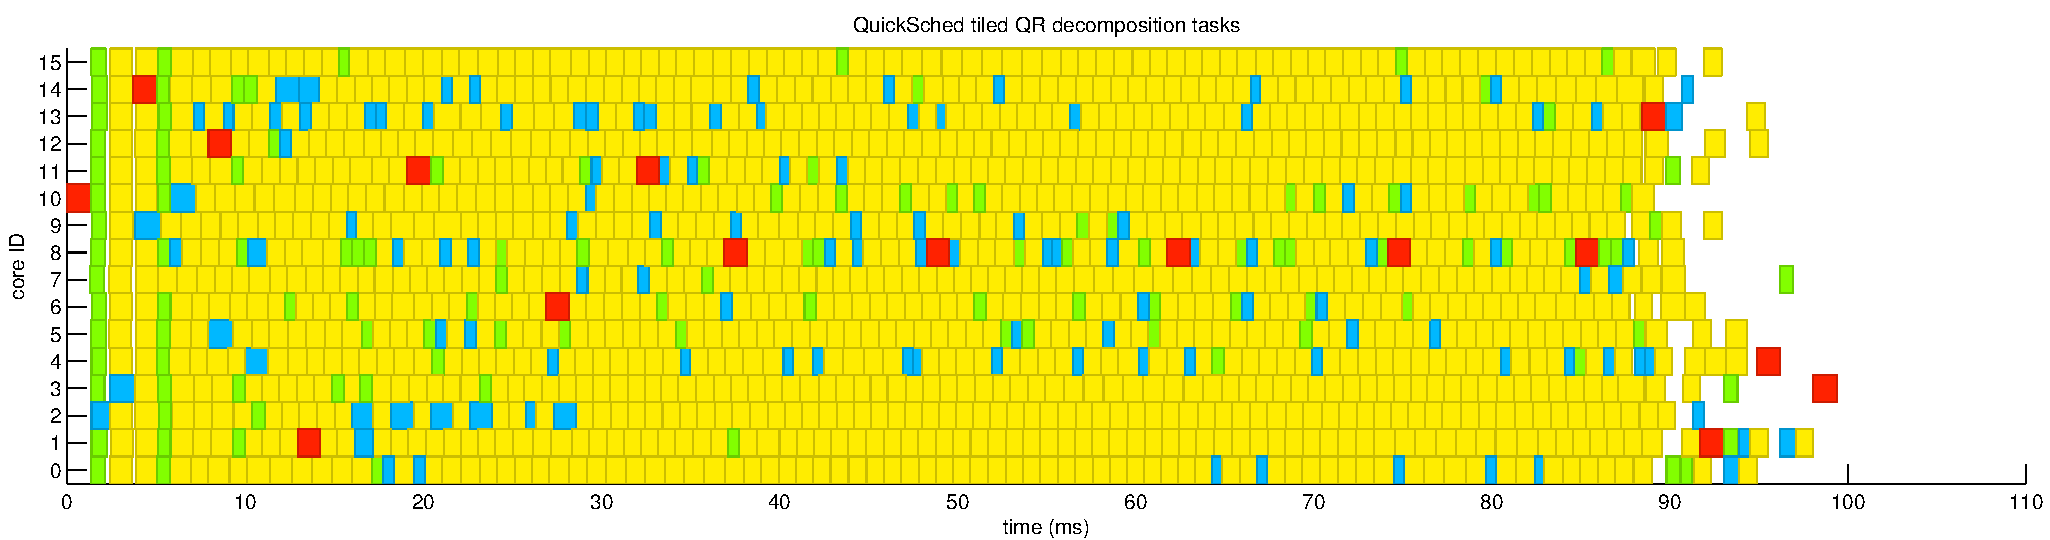
\epsfig{file=figures/tasks_qr.pdf,width=0.9\textwidth}}
    \centerline{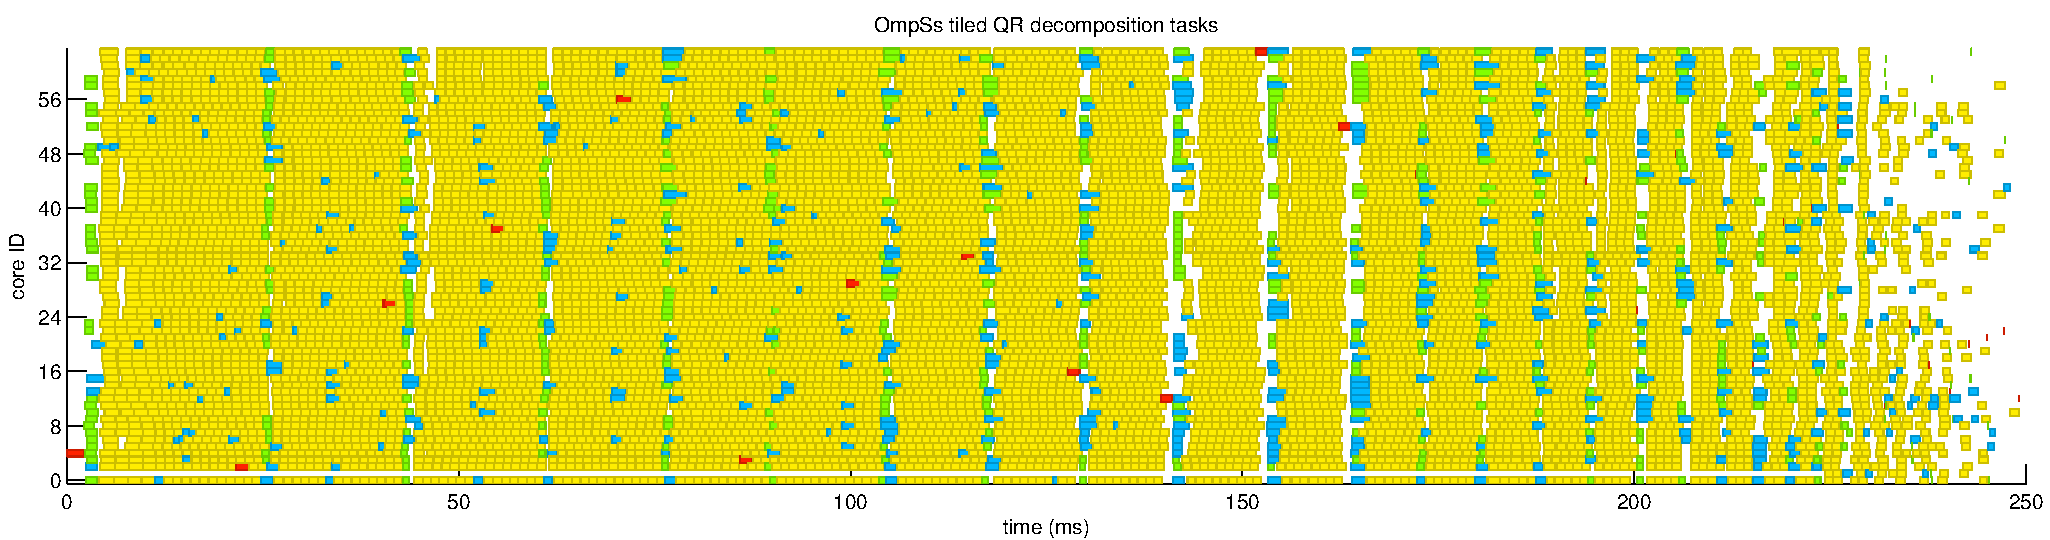
\epsfig{file=figures/tasks_qr_ompss.pdf,width=0.9\textwidth}}
    \caption{Task scheduling in QuickSched (above) and OmpSs (below)
        for a $2048\times 2048$ matrix on 64 cores.
        The task colors correspond to those in \fig{QR}.}
    \label{fig:QRTasks}
\end{figure}


\subsection{Task-Based Barnes-Hut N-Body Solver}

The Barnes-Hut tree-code is an algorithm to approximate the
solution of an $N$-body problem, i.e.~computing all the
pairwise interactions between a set of $N$ particles,
in \oh{N\log N} operations, as opposed to the \oh{N^2}
naive direct computation.
The algorithm is based on a recursive octree decomposition:
Starting from a cubic cell containing all the particles,
the cell is recursively bisected along all three spatial dimensions,
resulting in eight sub-cells, until the number of particles
per cell is smaller than some limit $n_\mathsf{max}$.

The particle interactions can also be formulated recursively:
Given a particle and a set of particles in a cell,
if the particle and cell
are sufficiently well separated, the particle-cell interactions
are approximated by interacting the particle with the cell's
center of mass.
If the particle and the cell are too close, and the cell
has sub-cells, i.e.~it contained more than $n_\mathsf{max}$
particles and was split in the recursive octree decomposition,
then the particle is interacted with each of the sub-cells
recursively.
Finally, if the cell is not split, i.e.~it is a leaf cell
in the octree, then the particle is interacted with all
particles in the cell, except for the particle itself if
it is in the same cell.
This operation is performed for each particle, starting
with the root-level cell containing all the particles.

The cells themselves are implemented using the following 
data structure:
\begin{center}\begin{minipage}{0.9\textwidth}
    \begin{lstlisting}
struct cell {
  double loc[3], h[3], com[3], mass;
  int split, count;
  struct part *parts;
  struct cell *progeny[8];
  qsched_res_t res;
  qsched_task_t task_com;
  };
    \end{lstlisting}
\end{minipage}\end{center}
\noindent where {\tt loc} and {\tt h} are the location
and size of the cell, respectively.
The {\tt com} and {\tt mass} fields represent the cell's
center of mass, which will be used in the particle-cell interactions.
The {\tt res} filed is the hierarchical resource representing
the cell's particles, and it is the parent resource of the cell
progeny's {\tt res}.
Similarly, the {\tt task\_com} is a task handle to
compute the center of mass of the cell's particles, and 
it depends on the {\tt task\_com} of all the progeny if
the cell is split.
{\tt parts} is a pointer to an array of {\tt count} 
particle structures, which contain all the particle
data of the form:
\begin{center}\begin{minipage}{0.9\textwidth}
    \begin{lstlisting}
struct part {
  double x[3], a[3], mass;
  int id;
  };
    \end{lstlisting}
\end{minipage}\end{center}
\noindent i.e.~the particle position, acceleration, mass,
and ID, respectively.

The particle data is sorted hierarchically, following the
octree structure.
Unlike in many codes, where the leaves store an array of
pointers to the underlying particles, the cells, at all
levels, store only a pointer to the first of their own particles,
and the total number of particles.
The current approach, illustrated in \fig{CellParts} is not
only more compact, it also allows a direct and more cache-efficient access
to the list of particles for any inner node of the tree.
The cost of sorting the particles, with a recursive
partitioning similar to QuickSort \cite{ref:Hoare1962},
is in \oh{N\log N}.

\begin{figure}
    \centerline{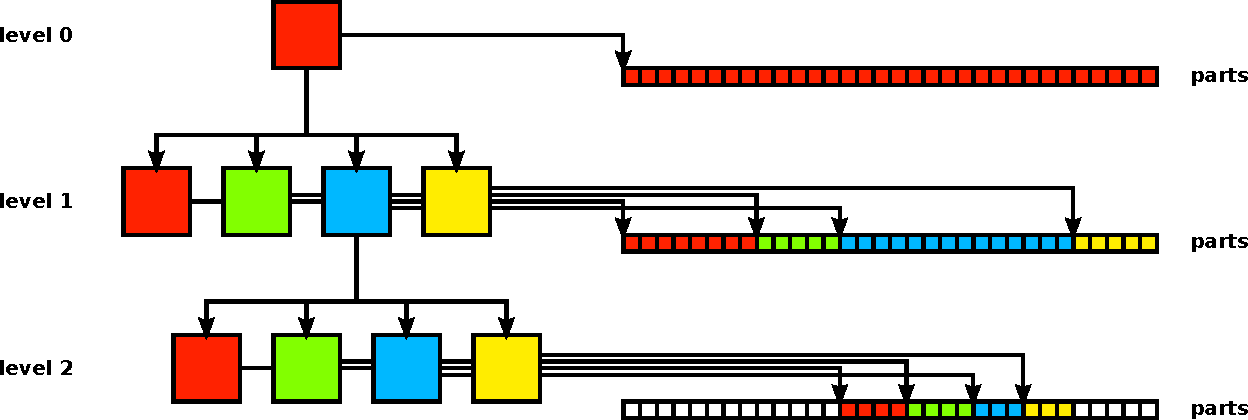
\epsfig{file=figures/CellParts.pdf,width=0.9\textwidth}}
    \caption{Hierarchical ordering of the particle data structures
    (right) according to their cell (left).
    Each cell has a pointer to the first of its particles (same color
    as cells) in the same global parts array.}
    \label{fig:CellParts}
\end{figure}

The task-based implementation will consist of four
types of tasks:
\begin{itemize}
    \item {\em Self}-interactions in which all particles
        in a single cell interact with all other particles in the
        same cell,
    \item {\em Particle-particle} pair interactions in which
        all particles in a cell interact with all
        particles in another cell,
    \item {\em Particle-cell} pair interactions in which
        all particles in one cell are interacted with the
        center of mass of another cell, and
    \item {\em Center of mass} tasks, which compute
        the center of mass of a single cell either from
        the sum of the centers of mass of its sub-cells
        if it has been split, or directly from the
        particles otherwise.
\end{itemize}

\begin{figure}
\begin{center}\begin{minipage}{0.9\textwidth}
    \begin{lstlisting}
enum { tSELF , tPAIR_PP , tPAIR_PC , tCOM };
void make_tasks ( struct qsched *s , struct cell *ci , struct cell *cj ) {
  int j, k;
  qsched_task_t tid;
  struct cell *data[2];
  if ( cj == NULL ) {
    if ( ci->split && ci->count > n_task )
      for ( j = 0 ; j < 8 ; j++ ) {
        make_tasks( s , ci->progeny[j] , NULL );
        for ( k = j+1 ; k < 8 ; k++ )
          make_tasks( s , ci->progeny[j] , ci->progeny[k] );
        }
    else {
      tid = qsched_addtask( s , tSELF , qsched_flags_none ,
        &ci , sizeof(struct cell *) , ci->count*ci->count );
      qsched_addlock( s , tid , ci->res );
      if ( ci->split )
        qsched_addunlock( s , ci->com , tid );
      }
    }
  else if ( ci and cj are well separated ) {
      data[0] = ci; data[1] = cj;
      tid = qsched_addtask( s , tPAIR_PC , qsched_flags_none ,
        data , sizeof(struct cell *)*2 , ci->count );
      qsched_addlock( s , tid , ci->res );
      qsched_addunlock( s , cj->com , tid );
      data[0] = cj; data[1] = ci;
      tid = qsched_addtask( s , tPAIR_PC , qsched_flags_none ,
        data , sizeof(struct cell *)*2 , cj->count );
      qsched_addlock( s , tid , cj->res );
      qsched_addunlock( s , ci->com , tid );
      }
  else if ( ci->split && cj->split && 
     ci->count*cj->count > n_task*n_task )
    for ( j = 0 ; j < 8 ; j++ )
      for ( k = 0 ; k < 8 ; k++ )
        make_tasks( s , ci->progeny[j] , cj->progeny[k] );
  else {
    data[0] = ci; data[1] = cj;
    tid = qsched_addtask( s , tPAIR_PP , qsched_flags_none ,
      data , sizeof(struct cell *)*2 , ci->count*cj->count );
    qsched_addlock( s , tid , ci->res );
    qsched_addlock( s , tid , cj->res );
    if ( ci->split && cj->split ) {
      qsched_addunlock( s , ci->com , tid );
      qsched_addunlock( s , cj->com , tid );
      }
    }
  }
    \end{lstlisting}
\end{minipage}\end{center}
    \caption{C-like pseudo-code for recursive task creation
        for the Barnes-Hut tree-code.}
    \label{fig:MakeTasks}
\end{figure}

These tasks can be created recursively over the cell hierarchy
as shown in the function {\tt make\_tasks} in \fig{MakeTasks}.
The function is called on the root cell with the root cell
and {\tt NULL} as its two cell parameters.
The function recurses as follows:
\begin{itemize}
    \item If called with a single (line~6), split (line~7) cell,
        recurse over all the cell's sub-cells (line~9), and all
        pairs of the cell's sub-cells (line~11),
    \item If called with a single unsplit cell (line~13),
        create a self-interaction task on that cell (line~14),
    \item If called with two cells that are sufficiently well
        separated (line~21), create two particle-cell pair
        interactions (lines~23 and~28) over both cells in
        opposite orders, which depend on the center of mass
        task of each cell,
    \item If called with two cells that are not well
        separated and both cells are split (line~33),
        recurse over all pairs of sub-cells spanning
        both cells (line~37), and
    \item If called with two cells that are not well separated
        and either of the cells are not split, create
        a particle-particle pair task over both cells.
\end{itemize}
\noindent where every interaction task additionally locks
the cells on which it operates (lines~16, 25, 30, and 42--43).

In order to prevent generating
a large number of very small tasks, the task generation only recurses
if the cells contain more than a minimum number $n_\mathsf{task}$
of threads each (lines~7 and~34).
The tasks themselves are then left to recurse over the sub-trees,
which is why in these cases, the tasks are made to depend on the
center of mass tasks (lines~17--18 and~41--47)
which may be used in the ensuing interactions.

\begin{figure}
\begin{center}\begin{minipage}{0.9\textwidth}
    \begin{lstlisting}
void comp_com ( struct cell *c ) {
  int j, k;
  c->com[0] = 0.0; c->com[1] = 0.0; c->com[2] = 0.0;
  c->mas = 0.0;
  if ( c->split )
    for ( k = 0 ; k < 8 ; k++ ) {
      struct cell *cp = c->progeny[k]
      for ( j = 0 ; j < 3 ; j++ ) c->com[j] += cp->com[j]*cp->mass;
      c->mass += cp->mass;
      }
  else
    for ( k = 0 ; k < 8 ; k++ ) {
      struct part *p = &c->parts[k];
      for ( j = 0 ; j < 3 ; j++ ) c->com[j] += p->x[j]*p->mass;
      c->mass += p->mass;
      }
  c->com[0] /= c->mass; c->com[1] /= c->mass; c->com[2] /= c->mass; 
  }

void comp_self ( struct cell *c ) {
  int j, k;
  if ( c->split )
    for ( j = 0 ; j < 8 ; j++ ) {
      comp_self( c->progeny[j] );
      for ( k = j+1 ; k < 8 ; k++ )
        comp_pair( c->progeny[j] , c->progeny[k] );
      }
  else
    for ( j = 0 ; j < c->count ; j++ )
      for ( k = j+1 ; k < c->count ; k++ )
        interact c->parts[j] and c->parts[k].
  }

void comp_pair ( struct cell *ci , struct cell *cj ) {
  int j, k;
  if ( ci and cj well separated ) {
    comp_pair_pc( ci , cj );
    comp_pair_pc( cj , ci );
    }
  else if ( ci->split && cj->split )
    for ( j = 0 ; j < 8 ; j++ )
      for ( k = 0 ; k < 8 ; k++ )
        comp_pair( ci->progeny[j] , cj->progeny[k] );
  else
    for ( j = 0 ; j < ci->count ; j++ )
      for ( k = 0 ; k < cj->count ; k++ )
        interact ci->parts[j] and cj->parts[k].
  }

void comp_pair_cp ( struct cell *ci , struct cell *cj ) {
  int k;
  for ( k = 0 ; k < ci->count ; k++ )
    interact ci->parts[k] and cj center of mass.
  }
    \end{lstlisting}
\end{minipage}\end{center}
    \caption{Task functions for the Barnes-Hut tree-code.}
    \label{fig:BHTasks}
\end{figure}

The functions for the task themselves are relatively
straight-forward and shown in \fig{BHTasks}, and the
execution function can be written as:
\begin{center}\begin{minipage}{0.9\textwidth}
    \begin{lstlisting}
void exec_fun ( int type , void *data ) {
  struct cell **cells = (struct cell **)data;
  switch ( type ) {
    case tSELF:
      comp_self( cells[0] );
      break;
    case tPAIR_PP:
      comp_pair( cells[0] , cells[1] );
      break;
    case tPAIR_PC:
      comp_pair_pc( cells[0] , cells[1] );
      break;
    case tCOM:
      comp_com( cells[0] );
      break;
    default:
      error( "Unknown task type." );
    }
  }
    \end{lstlisting}
\end{minipage}\end{center}


This Barnes-Hut tree-code was used to approximate the gravitational
N-Body problem for 1\,000\,000 particles with random coordinates
in $[0,1]^3$.
The parameters $n_\mathsf{max}=100$ and $n_\mathsf{task}=5000$
were used to generate the tasks, and cell pairs were considered
well separated if not directly adjacent.
Using the above scheme generated 161\,613 tasks, of which
512 self-interaction tasks, 18\,532 particle-particle interaction
task, 105\,120 particle-cell interaction tasks, and 37\,449
center of mass tasks.
A total of 179\,632 dependencies were generated, along with
142\,696 locks on 37\,449 resources.

For these tests, OpenMP parallelism was used and resource
re-owning was switched off.
Resource ownership was attributed by dividing the global
{\tt parts} array by the number of queues and assigning each cell's
{\tt res} to the fraction of the {\tt parts} array to which
the first of its own {\tt parts} belong.
The interactions  computed 10 times for each number of
cores, and the average thereof taken for the scaling and
efficiency results in \fig{BHResults}.
The timings are for {\tt qsched\_run}, including the cost of
{\tt qsched\_start}, which does not run in parallel.
Setting up the scheduler, tasks, and resources took, in all
cases, an average of 51.3\,ms.

\begin{figure}
    \centerline{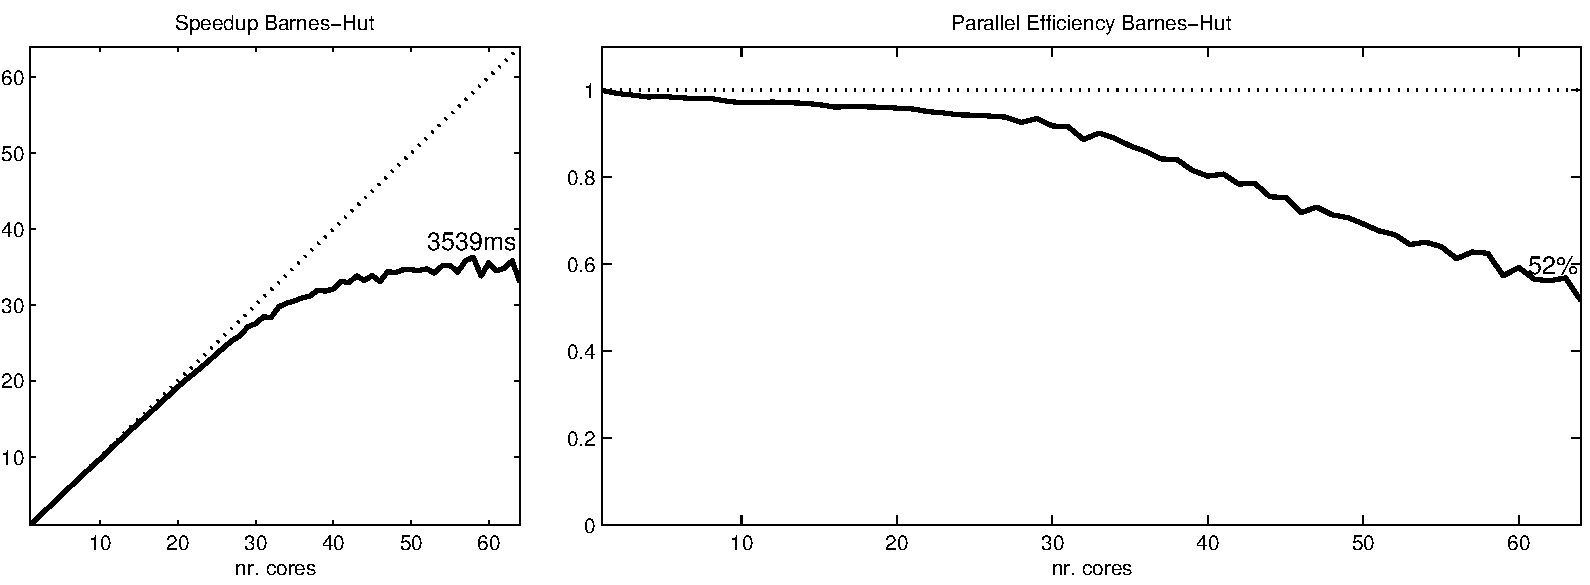
\epsfig{file=figures/BH_scaling.pdf,width=0.9\textwidth}}
    \caption{Strong scaling and parallel efficiency of the Barnes-Hut tree-code
        computed over 1\,000\,000 particles.
        Solving the N-Body problem takes 3.3\,s, achieving 60\% parallel
        efficiency, over all 64 cores.
        }
    \label{fig:BHResults}
\end{figure}

Unlike the QR decomposition, the results scale well only to
32 cores, achieving 90\% parallel efficiency, and then
level off for increasing numbers of cores.
This, however, is not a problem of the task-based parallel
algorithm, or of QuickSched, but of the memory bandwidth
of the underlying hardware.
\fig{BHTasks} shows the accumulated cost of each task type and of 
QuickSched over the number of cores.
At 64 cores, the scheduler overheads account for only 4.7\% of
the total computational cost, whereas,
as of 30 cores, the cost of both pair types grow by up to
50\%.
This is most probably due to memory bandwidth restrictions, as
the cost of the self interaction tasks, which do twice as much
computation per memory access, only grow by up to 15\%.

\begin{figure}
    \centerline{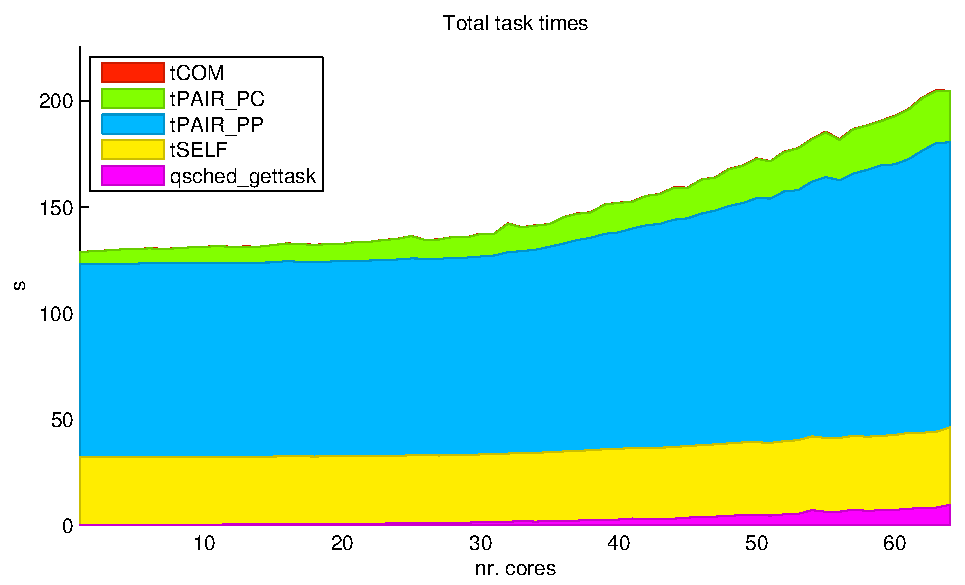
\epsfig{file=figures/BH_times.pdf,width=0.8\textwidth}}
    \caption{Accumulated cost of each task type and of the overheads
        associated with {\tt qsched\_gettask}.
        As of $\sim 30$ cores, the cost of both pair interaction task
        types grow by up to 50\%.
        The cost of the self interactions, which entail twice as much
        computation per memory access, grow only by at most 15\%.
        The scheduler overheads make up less than 5\% of the total
        time.
        }
    \label{fig:BHTimes}
\end{figure}


\section{Discussion and Conclusions}

The task scheduler described in the previous sections, QuickSched,
differs from existing task-based programming schemes
in a number of ways.
The most obvious such difference is the addition of {\em conflicts},
modeled using exclusive locks on hierarchical resources.
This extension to the standard dependencies-only model
of task-based parallelism allows for more complex task relations,
such as in the Barnes-Hut tree-code described earlier.

Another significant difference is that the tasks, their
dependencies, and their conflicts must be described
{\em explicitly} before the parallel computation starts.
This as opposed to implicit dependencies generated
by task spawning, e.g.~as in Cilk, or to extracting the
dependencies from the task parameters, e.g.~in QUARK or OmpSs.
Explicitly defining dependencies has the advantage that 
more elaborate dependency structures can be generated.
Furthermore, knowing the structure of the entire task
graph from the start of the computation provides valuable
information when scheduling the tasks, e.g.~using the 
critical path along the dependencies to compute the
task weight.

Finally, as opposed to the most other task-based
programming environments which rely on compiler extensions
and/or code pre-processors, QuickSched operates as a regular
C-language library, based on standard parallel functionality
provided by OpenMP and/or {\tt pthreads}.
This ensures a maximum amount of portability on existing
and future architectures.
The interfaces are also kept as simple
as possible in order to reduce the burden on the programmer
when implementing task-based codes.

The QuickSched library itself is remarkably simple, consisting of
less than 3\,000 lines of code, including comments.
Both examples, which are distributed with QuickSched,
require less than 1\,000 lines of code each.

In both examples, QuickSched performs extremely well, even
on a large number of shared-memory cores.
This performance is due, on the one hand, to the
division of labor between the scheduler and the queues,
and on the other hand due to the simple yet efficient
algorithms for task selection and resource locking.
The task weighting based on the length of the critical
path of the dependencies delivers, in the examples shown,
good parallel efficiency.

There are several possible improvements to QuickSched which
have not been addressed in this paper.
The most obvious of which are the following:
\begin{itemize}
    \item {\em Priorities}: The current implementation of
        QuickSched does not take the resource locks into
        account when selecting tasks in the queues,
    \item {\em Work-stealing}: During work-stealing, the
        queues are probed in a random order although
        the total relative cost of the tasks in the queue,
        as well as the length of their critical paths are
        known,
    \item {\em Costs}: The size of the resources used by
        a task are currently not taken into account when
        assigning it to the queues in {\tt qsched\_enqueue},
        or when approximating the cost of a task.
\end{itemize}

QuickSched is distributed under the GNU Lesser General Public Licence
v\,3.0 and is available for download via
\url{https://sourceforge.net/projects/quicksched/files/}.


% Acknowledgments
\begin{acks}
The author would like to thank Sam Townsend for implementing the
kernels in the task-based QR decomposition as part of his MSc Thesis
at Durham University.
The author also thanks Lydia Heck of the Institute for
Computational Cosmology at Durham University for providing access
to, and expertise on, the COSMA cluster used in the performance
evaluation.
\end{acks}

% Bibliography
\bibliographystyle{ACM-Reference-Format-Journals}
\bibliography{quicksched}
                             % Sample .bib file with references that match those in
                             % the 'Specifications Document (V1.5)' as well containing
                             % 'legacy' bibs and bibs with 'alternate codings'.
                             % Gerry Murray - March 2012

% History dates
\received{February 2007}{March 2009}{June 2009}

\end{document}
% End of v2-acmsmall-sample.tex (March 2012) - Gerry Murray, ACM


